\documentclass[conference]{IEEEtran}
\IEEEoverridecommandlockouts

\usepackage{cite}
\usepackage{amsmath,amssymb,amsfonts}
\usepackage{algorithmic}
\usepackage{graphicx}
\usepackage{dblfloatfix}
\usepackage{hyperref}
\usepackage{caption}
\usepackage{pifont}
\usepackage{textcomp}
\usepackage{multirow}
\usepackage[table,xcdraw]{xcolor}
\usepackage[strings]{underscore}

\graphicspath{{figures/}}
\newcommand{\cmark}{\ding{51}}
\newcommand{\xmark}{\ding{55}}
\def\BibTeX{{\rm B\kern-.05em{\sc i\kern-.025em b}\kern-.08emT\kern-.1667em\lower.7ex\hbox{E}\kern-.125emX}}

\begin{document}

\title{Multi-Label Speech Emotion Recognition Using 2D Convolutional Neural Networks}

\author{\IEEEauthorblockN{Brian Pho, Thomas Truong, Svetlana Yanushkevich}
\IEEEauthorblockA{\textit{Biometric Technologies Laboratory, Department of Electrical and Computer Engineering}\\
University of Calgary, Canada\\
\{brian.pho, thomas.truong, syanshk\}@ucalgary.ca}}

\maketitle

\begin{abstract}
Current speech emotion recognition systems often overlook the multi-label data that comes with databases. In this paper, we address the problem of whether machine learning can be used to detect multiple emotions in speech. We created a combined database consisting of four speech emotion-labeled databases, and we used it to train a 2D convolutional neural network to determine if the model could recognize multiple emotions in a speech sample. The model was able to classify the samples with an accuracy of 57.64\%. This shows that it is possible to apply machine learning to the problem of multi-label speech emotion recognition and to achieve a reasonable accuracy.\footnote{Code for this paper is available on Github at: \url{https://github.com/Brian-Pho/RVST598_Speech-Emotion-Recognition}}
\end{abstract}

\begin{IEEEkeywords}
multi-label, speech, emotion, recognition, neural networks
\end{IEEEkeywords}

\section{Introduction}
The field of affective computing studies the development of systems that can recognize, interpret, process, and simulate human affects. A subfield of affective computing that we are interested in is speech emotion recognition (SER). SER is the problem of recognizing which emotions are present in speech and SER has been approached in two ways:
\begin{itemize}
	\item Feature engineering
	\item Machine learning (ML)
\end{itemize}

\subsection{Literature Review}

Feature engineering is a method of manually extracting desired parameters from the data for use in  recognition. For audio, examples of parameters include pitch, energy, and Mel-Frequency Cepstral Coefficients (MFCC).\cite{Rybka2013} Nassif et al. \cite{Nassif2019} found that most researchers used the MFCC parameter for deep learning models but also recommended other parameters such as Linear Predictive Coding. 

Machine learning is a method of creating an artificial neural network that automatically extracts its own parameters for recognition. Examples include support vector machines (SVM), convolutional neural networks (CNN), and recurrent neural networks (RNN). Both approaches are not exclusive and a hybrid approach of feature engineering and machine learning results in better classification accuracy.\cite{Nassif2019}

A common example of combining both approaches is to convert an audio waveform into a spectrogram using the Short-Time Fourier Transform (STFT) and to feed the spectrogram into a neural network. Papers such as \cite{Engel2019}, \cite{Chen2018}, \cite{Badshah2019}, and \cite{Zhao2019} have demonstrated that this approach is successful for processing audio and for recognizing emotions in speech.

Current state-of-the-art SER has achieved an accuracy of 52.14\% for the case of speaker-independent, single-labeled emotions on the IEMOCAP database.\cite{Zhao2019} This result was achieved using a 2D CNN long short-term memory (LSTM) model where the audio waveform was converted into a log-Mel spectrogram and then fed into the model.

However, this model and most other models only consider a single emotion per speech sample and are often only trained on one or two databases. Kim et al. \cite{Kim2018a} is an exception as they consider the multi-label case of SER but they did not use machine learning and they used visual data on top of audio data. This paper extends upon current literature by considering the problem of multi-label SER using four databases to train and test a CNN.

The IEMOCAP \cite{busso_2008} and CREMA-D \cite{cao_2014} databases both include multiple labels for each speech sample but the data is discarded by considering the emotion with the majority of votes. We argue that discarding the non-majority votes results in a less realistic model of emotion classification due to not matching human performance and due to the loss of information by discarding votes.

\subsection{Proposed Approach}

We approach the problem of multi-label emotion classification by using a 2D CNN to classify speech samples into multiple emotions. We collected four databases: two with multi-label and single-label samples, and two with only single-label samples. We then combined the four databases into an a single database by processing all of the speech samples into log-Mel spectrograms. These log-Mel spectrograms were then fed into an eight-layer neural network consisting of four convolutional layers and four dense layers.

This paper is outlined as follows:
\begin{itemize}
	\item Section II details the methodology we use such as the how we combined the four databases and describes the architecture of the neural network.
	\item Section III describes and discusses the results from testing the neural network.
	\item Section IV concludes this paper and provides suggestions for future directions.
\end{itemize}

\bgroup
\def\arraystretch{2}
\begin{table*}
	\resizebox{\textwidth}{!}{%
		\begin{tabular}{|l|c|c|c|c|c|c|c|c|c|c|c|c|c|}
			\hline
			\multicolumn{1}{|c|}{} & \multicolumn{13}{c|}{\textbf{Emotions}} \\ \cline{2-14} 
			\multicolumn{1}{|c|}{\multirow{-2}{*}{\textbf{Databases}}} & \textbf{Neutral} & \textbf{Anger} & \textbf{Disgust} & \textbf{Fear} & \textbf{Happy} & \textbf{Sad} & \textbf{Surprise} & \textbf{Calm} & \textbf{Excitement} & \textbf{Frustration} & \textbf{Amused} & \textbf{Sleepy} & \textbf{Bored} \\ \hline
			\rowcolor[HTML]{F6F8FA} 
			\textbf{IEMOCAP} & \cmark & \cmark & \cmark & \cmark & \cmark & \cmark & \cmark & \xmark & \cmark & \cmark & \xmark & \xmark & \xmark \\ \hline
			\textbf{CREMA-D} & \cmark & \cmark & \cmark & \cmark & \cmark & \cmark & \xmark & \xmark & \xmark & \xmark & \xmark & \xmark & \xmark \\ \hline
			\rowcolor[HTML]{F6F8FA} 
			\textbf{TESS} & \cmark & \cmark & \cmark & \cmark & \cmark & \cmark & \cmark & \xmark & \xmark & \xmark & \xmark & \xmark & \xmark \\ \hline
			\textbf{RAVDESS} & \cmark & \cmark & \cmark & \cmark & \cmark & \cmark & \cmark & \cmark & \xmark & \xmark & \xmark & \xmark & \xmark \\ \hline
			\rowcolor[HTML]{F6F8FA} 
			\textbf{MSP-IMPROV} & \cmark & \cmark & \cmark & \cmark & \cmark & \cmark & \cmark & \xmark & \xmark & \xmark & \xmark & \xmark & \xmark \\ \hline
			\textbf{SAVEE} & \cmark & \cmark & \cmark & \cmark & \cmark & \cmark & \cmark & \xmark & \xmark & \xmark & \xmark & \xmark & \xmark \\ \hline
			\rowcolor[HTML]{F6F8FA} 
			\textbf{Emo-DB} & \cmark & \cmark & \cmark & \cmark & \cmark & \cmark & \xmark & \xmark & \xmark & \xmark & \xmark & \xmark & \cmark \\ \hline
			\textbf{EmoV-DB} & \cmark & \cmark & \cmark & \xmark & \xmark & \xmark & \xmark & \xmark & \xmark & \xmark & \cmark & \cmark & \xmark \\ \hline
		\end{tabular}%
	}
	\caption{Comparison of databases with their labeled emotions.}
	\label{dbEmoTable}
\end{table*}
\egroup


\section{Methodology}

We approach the problem of SER by preprocessing samples from four databases and then feeding those samples into a CNN. We preprocess the speech samples into log-Mel spectrogram to help the neural network extract features relevant to emotion recognition. This choice is based on previous work such as \cite{Engel2019} and \cite{Badshah2017}. The choice of using a CNN is also based on previous work where Balakrishnan et al. \cite{Balakrishnan2017} found that CNN-based models have superior performance compared to RNNs. Another justification for using CNNs is due treating the log-Mel spectrograms as images which CNNs have been shown to perform well on.\cite{Krizhevsky2012}

A high level overview of the data flow is shown in figure \ref{highLevelDataFlowDiagram} where samples flow through four stages of processing. The stages are detailed further into the methodology. Both the preprocessing steps and the CNN were implemented in Python using the Librosa \cite{McFee2015} and Keras \cite{Chollet2015} library respectively.

\subsection{Preprocessing}

To determine if a ML model can perform multi-label speech emotion recognition, we first need to obtain speech samples with their labeled emotion. We considered eight databases and chose four based on accessibility and the number of overlapping emotions. Table \ref{dbEmoTable} compares the set of emotions of each database which makes it easier to identify overlapping emotions. We chose four databases because it becomes more difficult to maintain consistency due to database variability. Databases can vary in
\begin{itemize}
	\item The set and number of labeled emotions
	\item The number of labels per sample
	\item The audio quality such as sampling rate and noise
	\item The spoken language
\end{itemize}
Given this variability, we chose the following four databases
\begin{enumerate}
	\item IEMOCAP \cite{busso_2008}
	\item TESS \cite{dupuis_2011}
	\item RAVDESS \cite{livingstone_2018}
	\item CREMA-D \cite{cao_2014}
\end{enumerate}

To control for the set and number of labeled emotions, we consider the following seven emotions for recognition
\begin{enumerate}
	\item Neutral
	\item Anger
	\item Disgust
	\item Fear
	\item Happy
	\item Sad
	\item Surprise
\end{enumerate}
We chose these seven emotions due to them being considered basic emotions by Ekman \cite{Ekman1992} and due to these seven being the most common among all databases. 

To control for the number of labels per sample, we mixed the multi-labeled data from the IEMOCAP and CREMA-D databases with the single-labeled data from the TESS and RAVDESS databases. We chose to mix of single- and multi- labeled data to increase the number of samples that the model can learn from and because the single-labels can be considered as special cases of multi-labeled data. However, we removed samples that were labeled with four or five emotions because we consider samples with that many emotions to be ambiguous and because outliers hinder a neural networks ability to learn. Outliers can cause large gradient updates which prevents a model from converging.

To control for the audio quality, we resampled all samples to 48 kHz, applied noise reduction to samples from the IEMOCAP and CREMA-D databases, and cropped all samples to 4.5 seconds. We used a kaiser filter for resampling and used spectral gating for noise reduction. We only applied noise reduction to the IEMOCAP and CREMA-D databases after listening to the audio. Lastly, we chose databases that are spoken in English to maintain language consistency.

We combined these four databases into a combined database to train, validate, and test the neural network. The combined database is detailed in figure \ref{combinedDb}.

\begin{figure*}[t]
	\centering
	\hspace{6mm}
	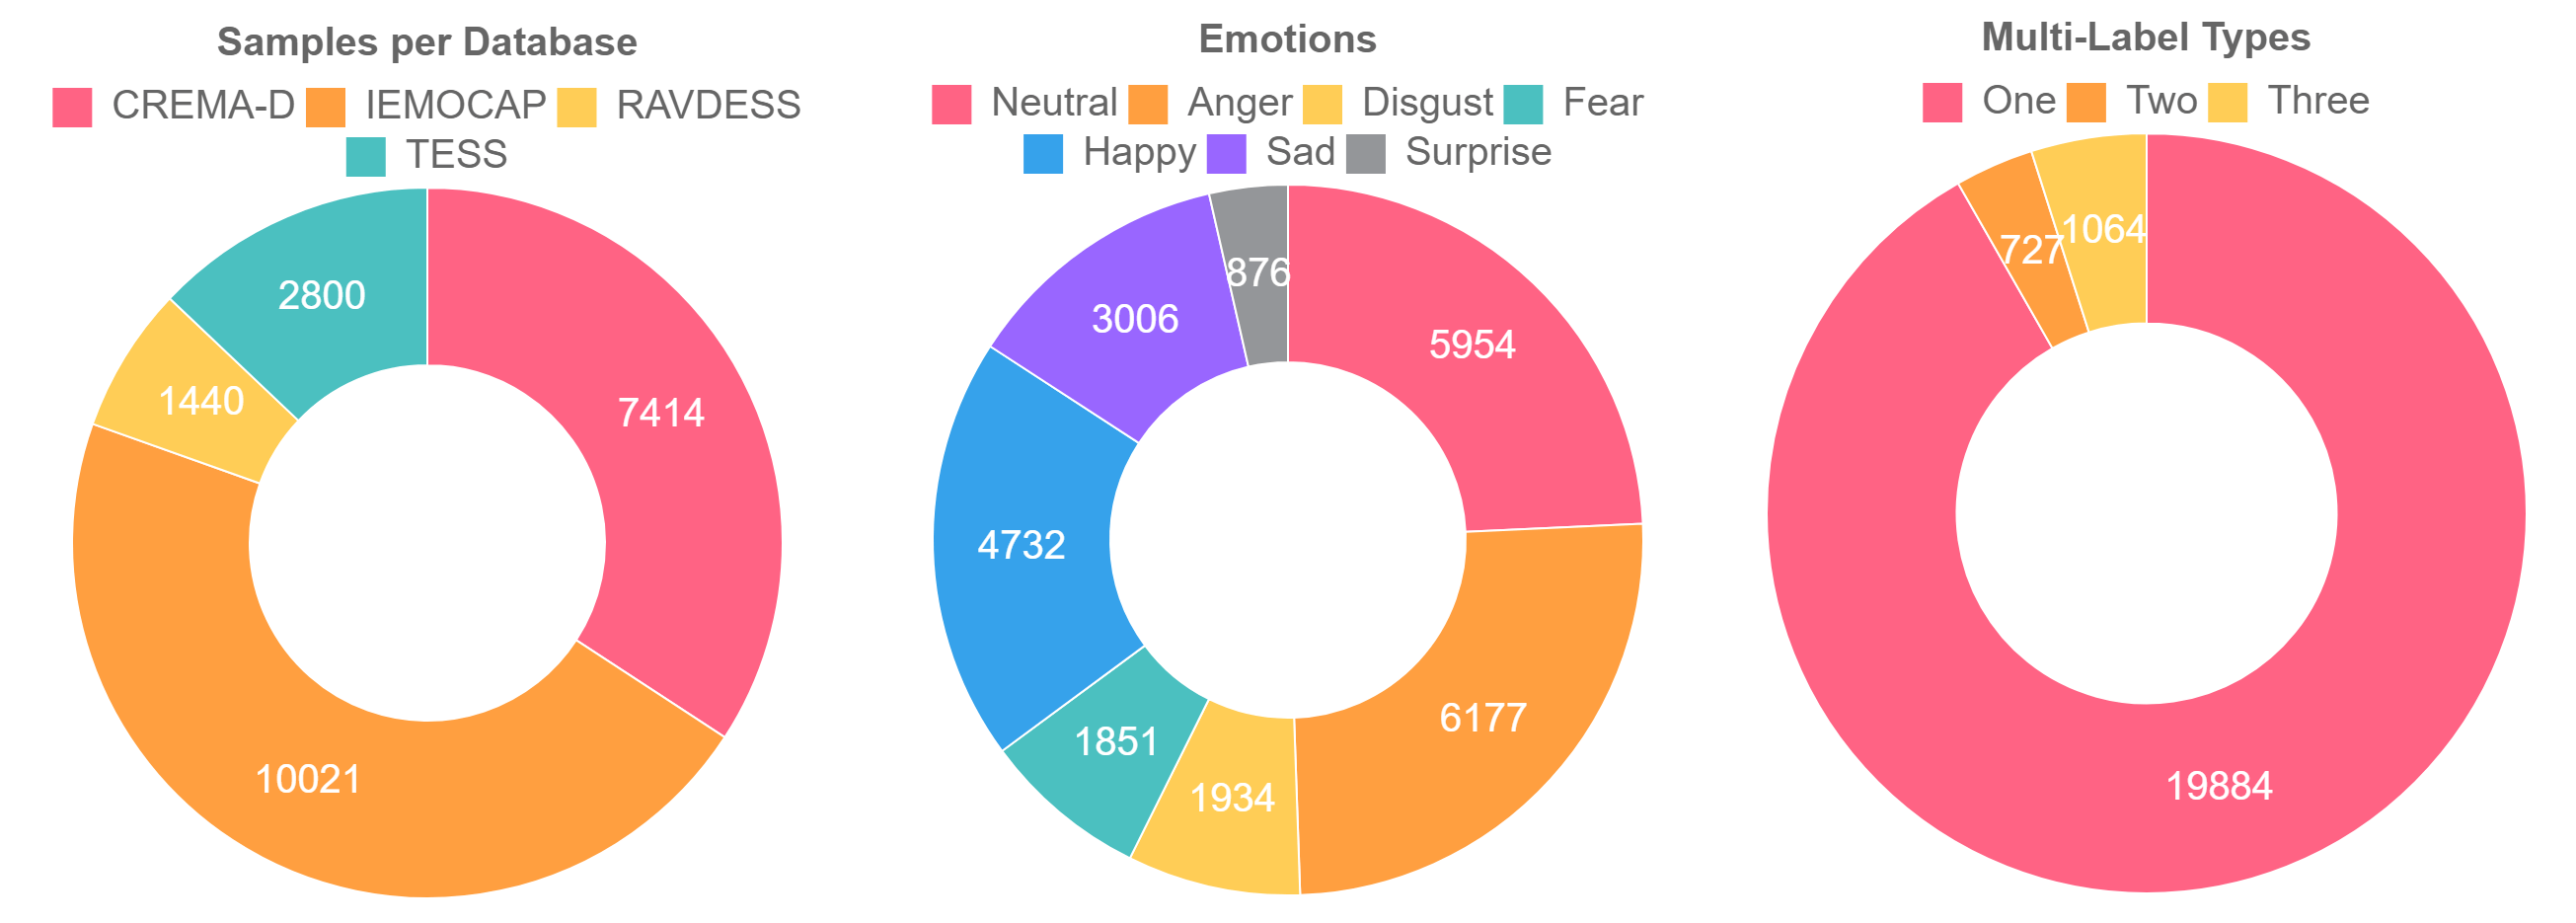
\includegraphics[width=\textwidth]{combined_db.png} 
	\caption{Proportions of each database, emotion, and label types in the combined database.}
	\label{combinedDb}
\end{figure*}

Each sample from a database would flow through the same preprocessing steps to maintain consistency across all samples. The detailed steps are described below.
\begin{enumerate}
	\item A sample starts as a raw waveform in the form of time series points specifying the amplitude at a certain point in time.
	\item The sample is then padded or cropped to the desired length of 4.5s. Shorter samples were zero-padded on the right tail. Longer samples were cropped and the extra information discarded.
	\item If the sample came from a database that we considered noisy, then a noise reduction filter was applied to the sample. We consider the IEMOCAP and CREMA-D databases to be noisy.
	\item The sample is then converted into a log-Mel spectrogram using the short-time Fourier transform (STFT) and Mel scale equation. The phase information was discard as it does not seem to hold relevant information. \cite{Kozakowski2017}
	\item The final step is to normalize the spectrograms to have values between negative one and one. This was done by using a min-max scaling function.
\end{enumerate}

The discrete-time STFT is defined in (\ref{stft}) where $x[n]$ is the discrete signal and $w[n]$ is the window function.

\begin{equation}
	\label{stft}
	\mathbf{STFT}\{x[n]\}(m,\omega) \equiv X(m,\omega) = \sum_{n=-\infty}^{\infty}x[n]w[n-m]e^{-j \omega n}
\end{equation}

The Mel scale is defined in (\ref{melScale}) where $f$ is the frequency in hertz and $m$ is mels.\cite{Oshaughnessy1990}

\begin{equation}
\label{melScale}
m = 2595 log_{10}(1 + \frac{f}{700})
\end{equation}

For the STFT, we used a window size of 3072 with a 75\% overlap. This choice is based on the work of Zhao et al. \cite{Zhao2019} where they also use 75\% overlap but with a smaller window size (2048) and they achieved excellent results. For the Mel spectrogram, we set the minimum frequency to 20 Hz and maximum frequency to 12 kHz with 200 Mel bins. The frequency range was chosen after experimenting with various ranges and selecting the range that resulted in visually clean spectrograms. The number of Mel bins was also chosen after experimentation as too few bins resulted in poor temporal resolution while too many bins resulted in poor frequency resolution. This is due to the Gabor limit which describes the trade-off between temporal and frequency resolution.

\begin{figure}[]
	\centering
	\hspace{6mm}
	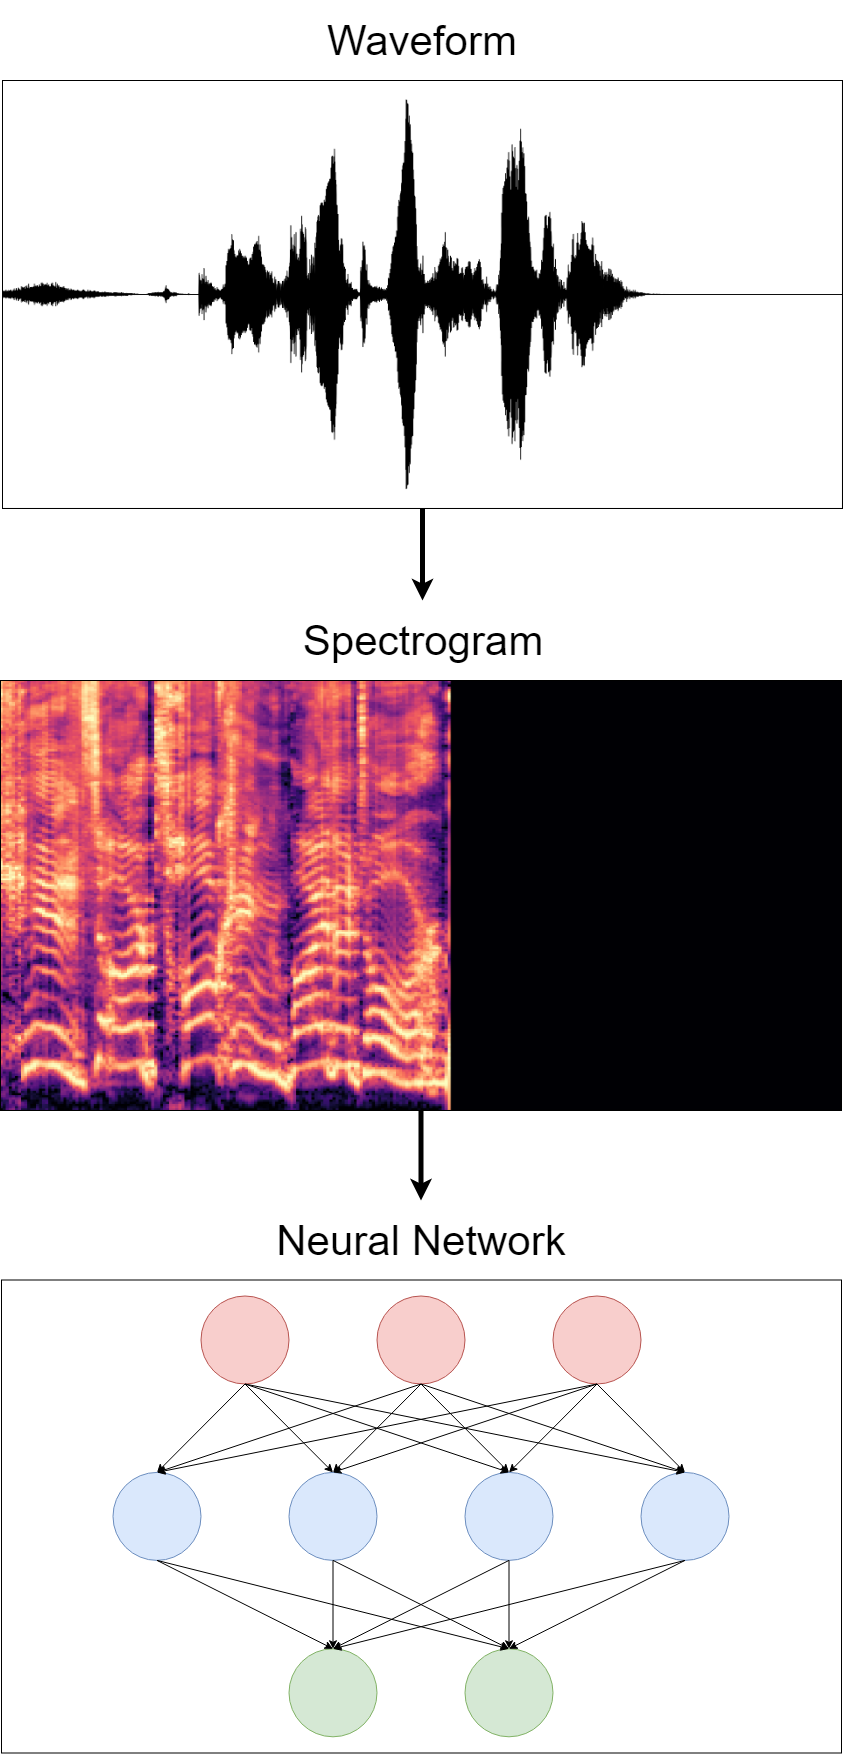
\includegraphics[width=\linewidth]{high_level_dataflow_diagram.png}
	\caption{High level overview of the processing stages that a speech sample goes through.}
	\label{highLevelDataFlowDiagram}
\end{figure}

\subsection{Neural Network}

\begin{figure*}[h!]
	\centering
	\hspace{6mm}
	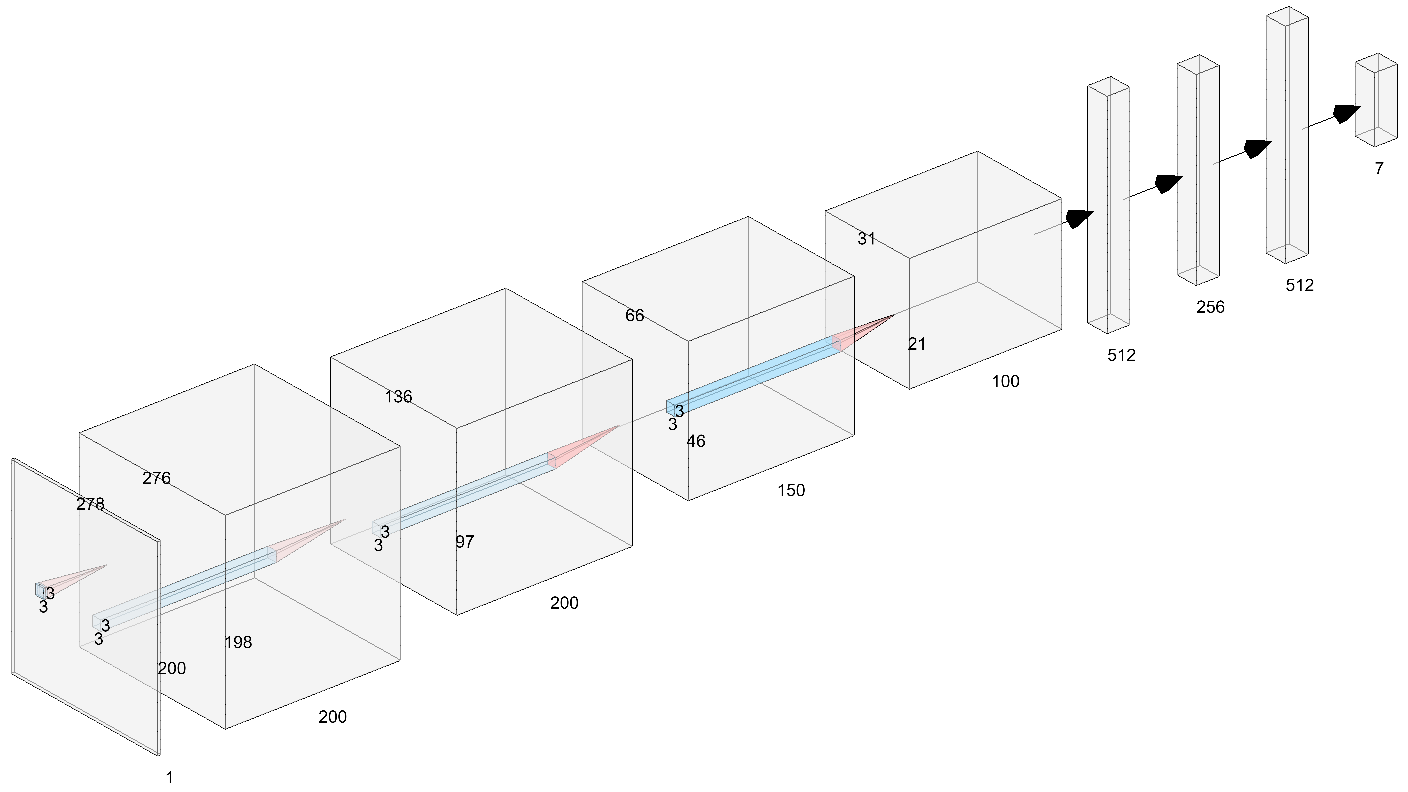
\includegraphics[width=\textwidth]{neural_network_architecture.png}
	\caption{Architecture for the speech emotion recognition network including the input layer and eight processing layers.}
	\label{neuralNetworkArchitecture}
\end{figure*}

After all of the databases were processed this way, the final combined database was fed into a neural network for training, validation, and testing. We constructed an eight layer neural network consisting of four convolutional layers and three dense layers. The network architecture is shown in figure \ref{neuralNetworkArchitecture}. The training process is described below.
\begin{itemize}
	\item We shuffled the combined database to make each input batch more uniform thus mitigating large gradient updates.
	\item We split the combined database into 80\% training, 10\% validation, and 10\% testing.
	\item We applied dropout to the dense layers and batch normalization to the convolutional layers to deal with overfitting. \cite{Srivastava2014}, \cite{Ioffe2015}
	\item We updated the model's hyperparameters based on the validation loss and accuracy to improve the model's accuracy and ability to generalize.
	\item We used class weights during training to address class imbalance.
\end{itemize}

Table \ref{modelHyperparams} describes the network hyperparameters and table \ref{trainHyperparams} describes the training hyperparameters.

\bgroup
\def\arraystretch{2}
\begin{table}[h!]
	\centering
	\caption{The model's hyperparameters.}
	\label{modelHyperparams}
	{%
		\begin{tabular}{|l|r|}
			\hline
			\textbf{Hyperparameter} & \textbf{Value} \\ \hline
			\rowcolor[HTML]{F6F8FA} 
			Input Dimensions & 278w x 200h x 1d \\ \hline
			Optimization Algorithm & Adam \\ \hline
			\rowcolor[HTML]{F6F8FA} 
			Loss Measure & Binary Cross-entropy \\ \hline
			Accuracy Metric & Categorical Cross-entropy \\ \hline
			\rowcolor[HTML]{F6F8FA} 
			Activation Function & Sigmoid \\ \hline
		\end{tabular}%
	}
\end{table}
\egroup

\bgroup
\def\arraystretch{2}
\begin{table}[h!]
	\centering
	\caption{The training hyperparameters.}
	\label{trainHyperparams}
	{%
		\begin{tabular}{|l|r|}
			\hline
			\textbf{Hyperparameter} & \textbf{Value} \\ \hline
			\rowcolor[HTML]{F6F8FA} 
			Epochs & 20 \\ \hline
			Batch Size & 32 \\ \hline
			\rowcolor[HTML]{F6F8FA} 
			Training Set & 17,341 \\ \hline
			Validation Set & 2,167 \\ \hline
			\rowcolor[HTML]{F6F8FA} 
			Testing Set & 2,167 \\ \hline
		\end{tabular}%
	}
\end{table}
\egroup

The final model was evaluated on the testing set by using average accuracy. The average accuracy is calculated from the confusion matrices shown in figure \ref{confusionMatrix}. The confusion matrices are calculated by comparing the true labels to the predicted labels for each emotion. There is a confusion matrix for each emotion due to the multi-label problem considering each emotion as independent.

We define accuracy as the unweighted average accuracy of all emotions and this is mathematically described in (\ref{aveacc}) where $n$ is the total number of emotions (7 in our case), $TP_{i}$ is the number of true positives for emotion $i$, $TN_{i}$ is the number of true negatives for emotion $i$, and $Total_{i}$ is the total number of predictions for emotion $i$.

\begin{equation}
\label{aveacc}
Accuracy = \frac{\sum_{i=1}^{n}\frac{TP_{i} + TN_{i}}{Total_{i}}}{n}
\end{equation}

In summary, we calculate the accuracy per emotion and then average over these accuracies to obtain the final accuracy. We chose this definition of accuracy so that we can compare our results to other papers that also use a similar measure of accuracy that is calculated from the confusion matrices.

\section{Results and Discussion}

After training the model, it was evaluated on the testing set to get the final accuracy. The final accuracy achieved was 57.64\%. Confusion matrices for each emotion are shown in Figure \ref{confusionMatrix} and comparisons to the current literature is shown in table \ref{litacccompare}.

\begin{figure*}[h!]
	\centering
	\hspace{6mm}
	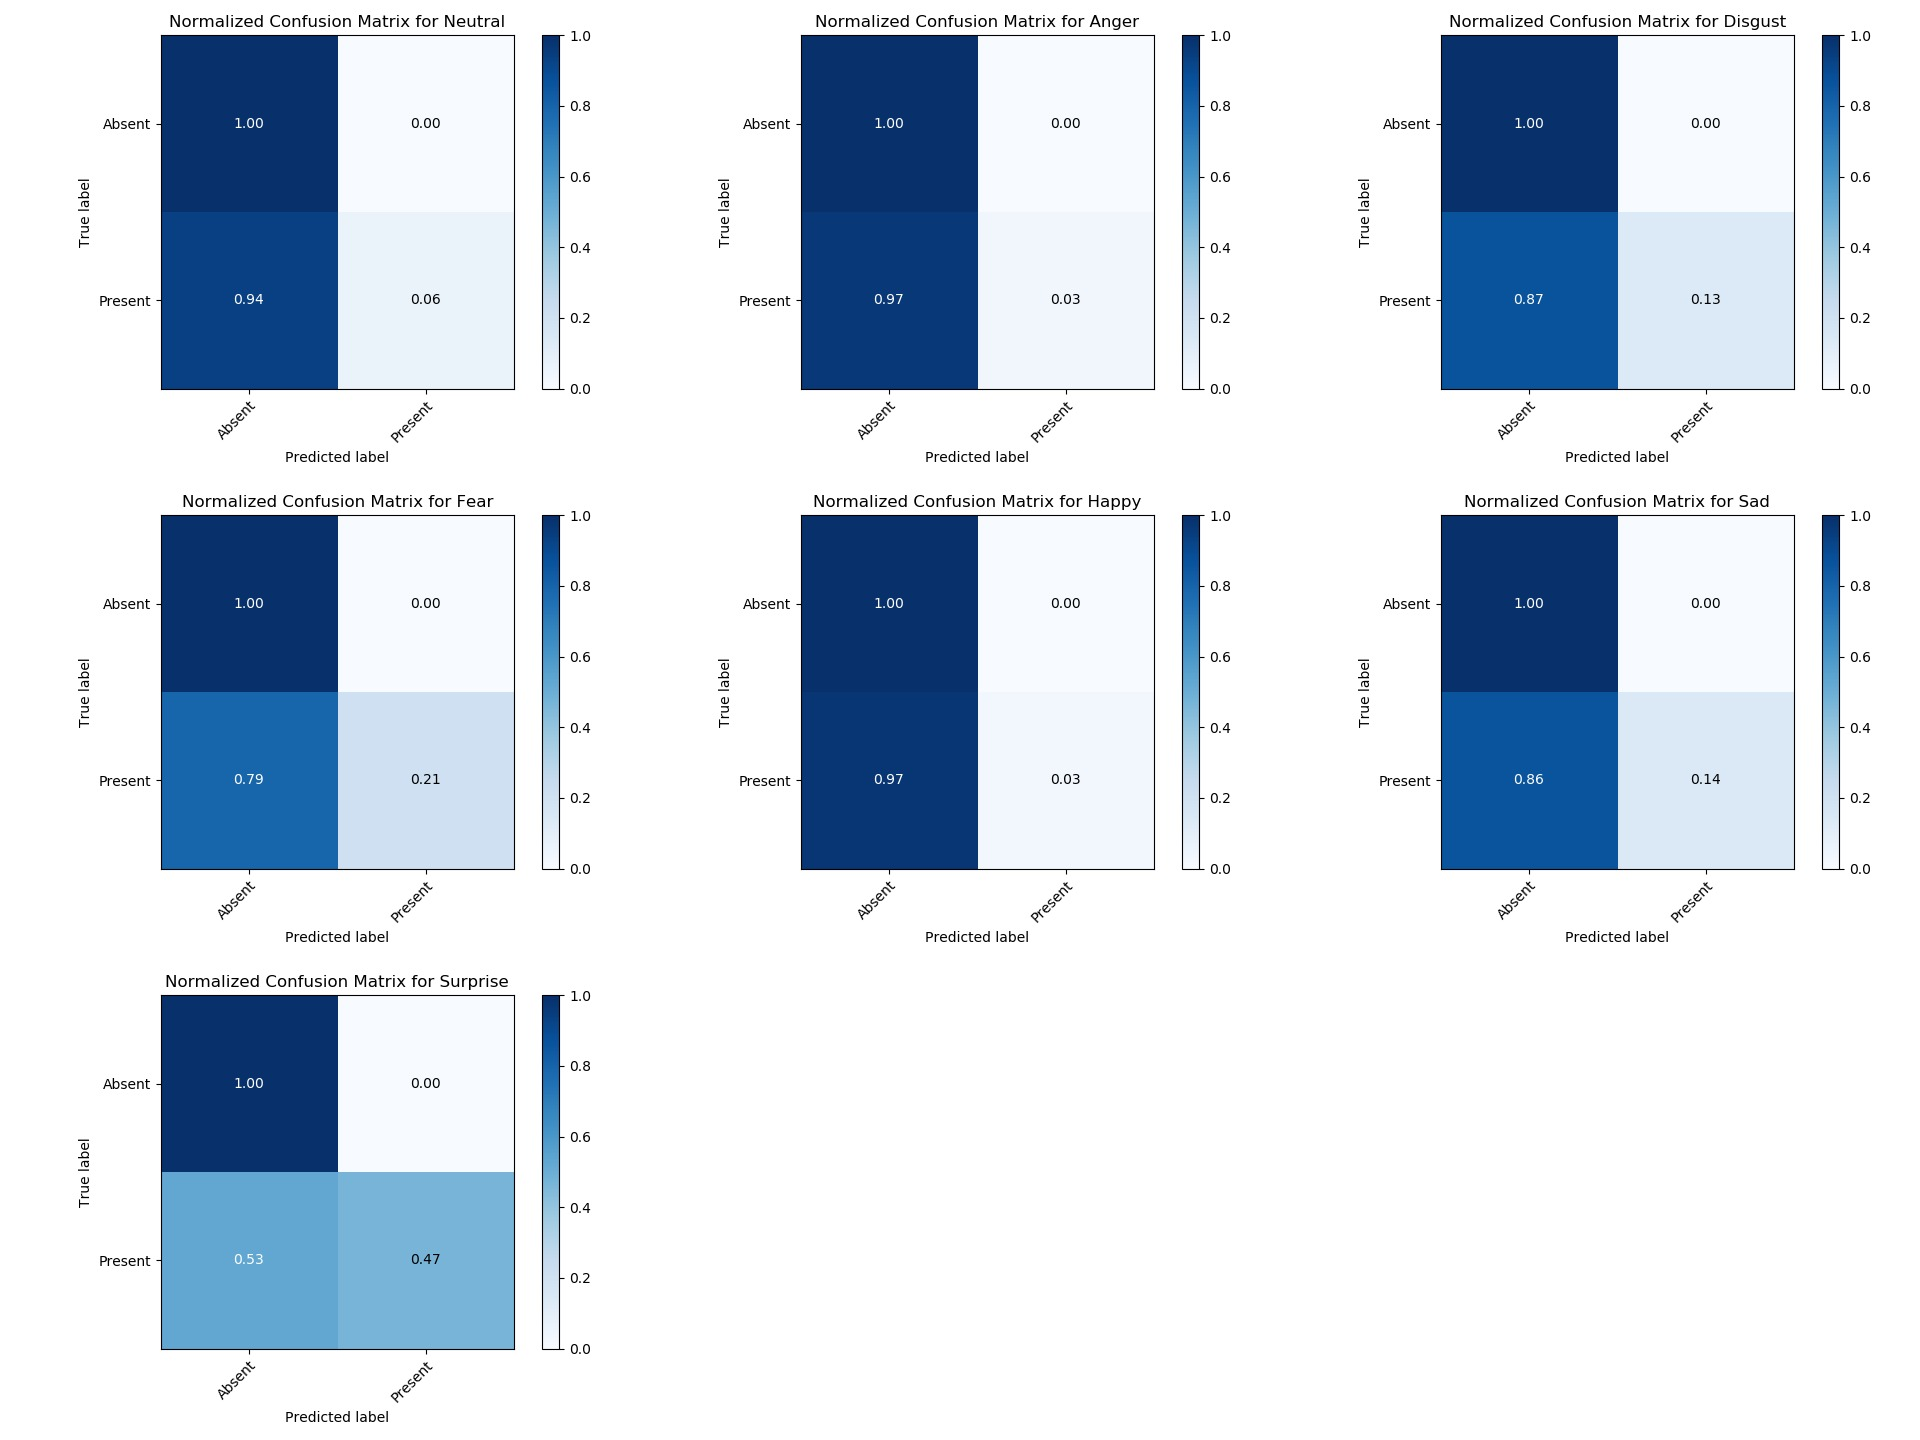
\includegraphics[width=\textwidth]{confusion_matrix.png}
	\caption{Confusion matrices for each emotion.}
	\label{confusionMatrix}
\end{figure*}

\bgroup
\def\arraystretch{2}
\begin{table}[]
	\centering
	\caption{Comparison of SER accuracy in literature.}
	\label{litacccompare}
	\begin{tabular}{|l|r|r|}
		\hline
		\multicolumn{1}{|c|}{\textbf{Research Work}} & \multicolumn{1}{c|}{\textbf{Method}} & \multicolumn{1}{c|}{\textbf{Accuracy (\%)}} \\ \hline
		\rowcolor[HTML]{F6F8FA}
		Zhao et al. \cite{Zhao2019} & CNN + LSTM & 52.1 \\ \hline
		Our Work & CNN & 57.6 \\ \hline
		\rowcolor[HTML]{F6F8FA}
		Etienne et al. \cite{Etienne2018} & CNN + LSTM & 61.7 \\ \hline
		Zhang et al. \cite{Zhang2019} & CNN & 63.9 \\ \hline
		\rowcolor[HTML]{F6F8FA}
		Fayek et al. \cite{Fayek2017} & CNN & 64.8 \\ \hline
		Yenigalla et al. \cite{Yenigalla2018} & CNN & 73.9 \\ \hline
		\rowcolor[HTML]{F6F8FA}
		Badshah et al. \cite {Badshah2019} & CNN & 84.3 \\ \hline
	\end{tabular}
\end{table}
\egroup

The results achieved in this paper do not reach the state-of-the-art accuracy achieved for the single-label case but this is the first attempt on the harder case of mutli-label using more data. So we conclude that it is possible to achieve a reasonable accuracy on the problem of multi-label speech emotion recognition by applying deep learning to the problem. 

In analyzing the confusion matrices, we see that the model predicts an emotion is absent in most of the samples with "surprise" being the exception. We suspect that "surprise" being an exception is due to the class imbalance that is shown in figure \ref{combinedDb}. The "surprise" class was the least represented class out of the seven classes and this makes the model predict it more due to the use of class weights. Class weights bias the model towards underrepresented classes in an attempt to balance classes but this seems to have affected the model's ability to learn.

\section{Conclusion and Future Work}

Overall, this paper presented a 2D CNN model that achieved an accuracy of 57.64\% on the problem of multi-label speech emotion recognition using four combined databases. We obtained this result by transforming raw speech samples into log-Mel spectrograms using the STFT and the Mel scale. The log-Mel spectrograms are then fed into an eight layer neural network for classification. While this result is a promising start, we suggest improvements that future work can build upon to improve the accuracy of the model and to expand the scope of emotions considered.

One limitation of this work is that we only accounted for seven emotions but recent research has suggested that there are more emotions such as boredom, shame, and triumph. \cite{Cordaro2018} However, one issue with expanding the set of considered emotions is the lack of databases with the labeled emotion.

Another limitation of this work is that all samples are spoken in English so the model is biased towards Anglophones. In theory, the basic emotions are universal across languages and cultures so incorporating databases spoken in different languages, such as the Emo-DB database, would help the model generalize across languages.\cite{Burkhardt2005}

The following list is a suggestion that future work could pursue:
\begin{itemize}
	\item Using more sophisticated neural network architectures such as LSTMs or using more databases.
	\item Incorporating the phase data from the STFT.
	\item Testing a binary relevance approach to this multi-label problem.
	\item Replacing the use of STFT with a wavelet transform.
\end{itemize}
Rana et al. \cite{Rana2016} has also shown that SER systems can be more robust by introducing noise into the samples which is another promising future direction.

\section*{Acknowledgment}
This work was funded by the Program for Undergraduate Research Experience (PURE) award granted by the University of Calgary.

\bibliographystyle{IEEEtran}
\bibliography{IEEEabrv,references}

\end{document}
